For the rows with $D\leq23$, \textbf{Lemma~\ref{lem:finite-k4}}
excludes a red $K_4$. Fix a vertex $v$ and let $N_r(v)$ be its set of red
neighbors. The red edges inside $N_r(v)$ form a triangle-free
graph. For any nonnegative weights $w_x$ on $N_r(v)$,
\[
 2\sum_{\substack{x,y\in N_r(v)\\xy\ {\rm red}}}w_xw_y
 \le \left(\sum_{x\in N_r(v)} w_x\right)^2.
\]
The sum on the left counts both orders of each edge. To see the
inequality, move the combined weight of two vertices with positive
weight that are nonadjacent in the red graph
onto the one with greater weighted neighbor sum. The edge sum does
not decrease, and iterating reduces the support of the weights to
a clique of size at most two. For two vertices it remains to use
$4w_xw_y\le(w_x+w_y)^2$. For a single vertex the left side is zero.
The weighted calculation uses
$w_x=1$, $w_x=b_{vx}$ and $w_x=1+b_{vx}$ for a red neighborhood rooted at $v$.
The square on the right includes two choices of the same vertex.


For $D=9$, let $u,v$ be the endpoints of two parallel marked
edges. The finite reduction gives
$|(N(u)\cup N(v))\setminus\{u,v\}|\in\{13,14\}$.
Since $uv$ is an edge, both roots lie in $N(u)\cup N(v)$, giving
$15\leq|N(u)\cup N(v)|\leq16$ in the reduced host.

For $D=13,15$, let $K$ consist of the vertices of a red triangle in
the host on the marked endpoints before regularization. Put
$E=\sum_{v\in K}(D-d_G(v)+j_v)$, and let $t$ and $q$ count the
vertices outside $K$ with at least two and exactly three neighbors
in $K$, respectively. We have $\sum_{v\in K}d_{\rm s}(v)=3D-E$.
Each of the three edges within $K$ contributes twice to this sum.
Hence there are $3(D-2)-E$ incidences between $K$ and its outside
neighbors. Counting distinct outside neighbors requires subtracting
one incidence at each of the $t$ vertices and one more at each of
the $q$ vertices. Including $K$, the number of vertices with a
neighbor in $K$ is therefore $N_+=3(D-1)-E-t-q$.

If a marked edge has an endpoint without a neighbor in $K$, its
other endpoint must be adjacent to a vertex cover of the red
triangle. This endpoint lies outside $K$ and has at least two
neighbors in $K$. Among its $D$ available incidences, at most
$D-2$ can meet vertices without a neighbor in $K$, and at most
$D-3$ if it has three neighbors in $K$. Thus the number
$m_{\rm out}$ of marked edges incident with vertices without a
neighbor in $K$ is at most $(D-2)t-q$. Summing marked degrees at
the $N_+$ vertices gives $2m-m_{\rm out}\leq DN_+$. Substitution
now gives
\[
 DE+2t+(D+1)q\le 3D(D-1)-2m.
\]
There are $u=3(D-2)-E-2t-q$ outside vertices with just one neighbor
in $K$. A marked edge between two of these vertices must join vertices
with different neighbors in $K$, since otherwise their edge could
have no joining edge to the opposite edge of the triangle. Thus the
marked graph on these $u$ vertices is tripartite. Each vertex has at
most $D-1$ marked incidences outside $K$, and the three classes span
at most $\lfloor\frac{u^2}{3}\rfloor$ distinct pairs joining different classes.
By \eqref{eq:multi-root-pair-budget}, at most
$w=\lfloor\frac{2D^2-m}{2D-1}\rfloor$ copies join any such pair.
At least $m-3D+3$ marks avoid $K$. Those with an endpoint having two
or three neighbors in $K$ account for at most $(D-2)t-q$. Consequently
\[
 m-3D+3\le (D-2)t-q+
 \min\left\{\left\lfloor\frac{(D-1)u}{2}\right\rfloor,
                  w\left\lfloor\frac{u^2}{3}\right\rfloor\right\}.
\]
When $N_+<\lceil\frac{2m}{D}\rceil$, some marked endpoint has no neighbor
in $K$. Choose an outside vertex $y$ with at least two neighbors in $K$
that sends the largest number $r$ of marked edges to vertices with no
neighbor in $K$. Then $1\le r\le D-2$, $m_{\rm out}\le tr$, and
$N_++tr\ge\lceil\frac{2m}{D}\rceil$, since every vertex of the reduced
host is a marked endpoint.

At a vertex incident with a repeated pair the number of extra copies
is at most
$j_{\max}=2D-3-\lceil\frac{m-2D+2}{D-1}\rceil$. Indeed, by
\eqref{eq:multi-root-pair-budget} a repeated pair has at least
$\lceil\frac{m-2D+2}{D-1}\rceil$ distinct neighbors outside its
endpoints. If the endpoints are $v,v'$, the same number is at most
$2D-2-j_v-j_{v'}$, and $j_{v'}\ge1$. It follows that the $r$
marked edges at $y$ have at least
$\max\{\lceil\frac{r}{w}\rceil,r-j_{\max}\}$ distinct endpoints
with no neighbor in $K$.

Fix one such endpoint $x$. Each marked edge between two vertices that
have just one neighbor in $K$ must meet $N_G(x)\cup N_G(y)$, because
it belongs to the same strong clique as $xy$. Each of its endpoints in
this union can meet at most $D-2$ such marks, having already used one
incidence at $K$ and one at $x$ or $y$. At least
$m-3D+3-(D-2)t$ marks join two vertices with just one neighbor in $K$.
At most $D-2-r$ of the vertices covering these marks can be neighbors of
$y$. Therefore $x$ is adjacent to at least
\[
 h=\max\left\{0,\left\lceil\frac{m-3D+3}{D-2}\right\rceil-t-(D-2-r)\right\}
\]
vertices having just one neighbor in $K$. All these edges at $x$
are unmarked. Counting their incidences at the other endpoints gives
\[
 \max\{\lceil\tfrac{r}{w}\rceil,r-j_{\max}\}\,h
 \le DN_+-(2m-m_{\rm out})\le DN_+-2m+tr .
\]
Thus, when $N_+<\lceil\frac{2m}{D}\rceil$, we retain $(E,t,q)$ only
if some $r$ satisfies these inequalities. In completing the host
we add only blue edges, and each new vertex is adjacent to at most
one vertex of $K$. Thus $t,q$ stay fixed and $E$ can only decrease.
For each retained pair $(t,q)$ we therefore include every integer $E$
from zero to the largest retained value. The resulting triples are
listed in \textbf{Figure~\ref{fig:finite-triangle-profiles}}. For example,
at $D=13$ the cell $(t,q)=(1,1)$ gives $E\in\{0,1,2\}$.
\begin{figure}[H]
\centering
\begingroup
\newcommand{\triangleneighbors}[1]{%
  \begin{tikzpicture}[x=.62cm,y=.62cm,baseline=(current bounding box.center)]
    \coordinate (a) at (0,0);
    \coordinate (b) at (1,.62);
    \coordinate (c) at (1,-.62);
    \coordinate (v) at (2.05,.20);
    \draw[line width=.6pt] (a)--(b)--(c)--cycle;
    \ifnum#1>0 \draw[densely dashed] (v)--(b);\fi
    \ifnum#1>1 \draw[densely dashed] (v)--(c);\fi
    \ifnum#1>2 \draw[densely dashed] (v)--(a);\fi
    \foreach \root in {a,b,c} {\fill (\root) circle[radius=1.3pt];}
    \draw[fill=white] (v) circle[radius=1.6pt];
  \end{tikzpicture}}
\begin{tabular}{cccc}
\triangleneighbors{0} & \triangleneighbors{1} & \triangleneighbors{2} & \triangleneighbors{3}\\
0 neighbors & 1 neighbor & 2 neighbors & 3 neighbors
\end{tabular}\par\medskip
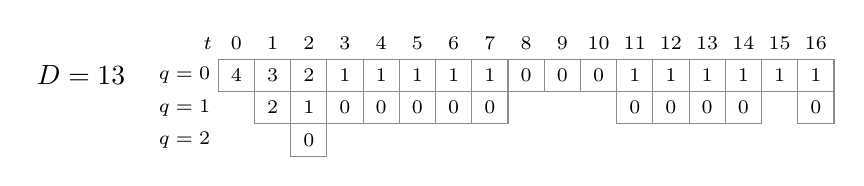
\begin{tikzpicture}[x=.46cm,y=.41cm,baseline=(current bounding box.center)]
\node[anchor=east] at (-2.8,-1) {$D=13$};
\node[anchor=east,font=\scriptsize] at (-.4,0) {$t$};
\node[font=\scriptsize] at (0,0) {$0$};
\node[font=\scriptsize] at (1,0) {$1$};
\node[font=\scriptsize] at (2,0) {$2$};
\node[font=\scriptsize] at (3,0) {$3$};
\node[font=\scriptsize] at (4,0) {$4$};
\node[font=\scriptsize] at (5,0) {$5$};
\node[font=\scriptsize] at (6,0) {$6$};
\node[font=\scriptsize] at (7,0) {$7$};
\node[font=\scriptsize] at (8,0) {$8$};
\node[font=\scriptsize] at (9,0) {$9$};
\node[font=\scriptsize] at (10,0) {$10$};
\node[font=\scriptsize] at (11,0) {$11$};
\node[font=\scriptsize] at (12,0) {$12$};
\node[font=\scriptsize] at (13,0) {$13$};
\node[font=\scriptsize] at (14,0) {$14$};
\node[font=\scriptsize] at (15,0) {$15$};
\node[font=\scriptsize] at (16,0) {$16$};
\node[anchor=east,font=\scriptsize] at (-.45,-1) {$q=0$};
\node[font=\scriptsize,draw=black!45,minimum width=.46cm,minimum height=.41cm,inner sep=0pt] at (0,-1) {$4$};
\node[font=\scriptsize,draw=black!45,minimum width=.46cm,minimum height=.41cm,inner sep=0pt] at (1,-1) {$3$};
\node[font=\scriptsize,draw=black!45,minimum width=.46cm,minimum height=.41cm,inner sep=0pt] at (2,-1) {$2$};
\node[font=\scriptsize,draw=black!45,minimum width=.46cm,minimum height=.41cm,inner sep=0pt] at (3,-1) {$1$};
\node[font=\scriptsize,draw=black!45,minimum width=.46cm,minimum height=.41cm,inner sep=0pt] at (4,-1) {$1$};
\node[font=\scriptsize,draw=black!45,minimum width=.46cm,minimum height=.41cm,inner sep=0pt] at (5,-1) {$1$};
\node[font=\scriptsize,draw=black!45,minimum width=.46cm,minimum height=.41cm,inner sep=0pt] at (6,-1) {$1$};
\node[font=\scriptsize,draw=black!45,minimum width=.46cm,minimum height=.41cm,inner sep=0pt] at (7,-1) {$1$};
\node[font=\scriptsize,draw=black!45,minimum width=.46cm,minimum height=.41cm,inner sep=0pt] at (8,-1) {$0$};
\node[font=\scriptsize,draw=black!45,minimum width=.46cm,minimum height=.41cm,inner sep=0pt] at (9,-1) {$0$};
\node[font=\scriptsize,draw=black!45,minimum width=.46cm,minimum height=.41cm,inner sep=0pt] at (10,-1) {$0$};
\node[font=\scriptsize,draw=black!45,minimum width=.46cm,minimum height=.41cm,inner sep=0pt] at (11,-1) {$1$};
\node[font=\scriptsize,draw=black!45,minimum width=.46cm,minimum height=.41cm,inner sep=0pt] at (12,-1) {$1$};
\node[font=\scriptsize,draw=black!45,minimum width=.46cm,minimum height=.41cm,inner sep=0pt] at (13,-1) {$1$};
\node[font=\scriptsize,draw=black!45,minimum width=.46cm,minimum height=.41cm,inner sep=0pt] at (14,-1) {$1$};
\node[font=\scriptsize,draw=black!45,minimum width=.46cm,minimum height=.41cm,inner sep=0pt] at (15,-1) {$1$};
\node[font=\scriptsize,draw=black!45,minimum width=.46cm,minimum height=.41cm,inner sep=0pt] at (16,-1) {$1$};
\node[anchor=east,font=\scriptsize] at (-.45,-2) {$q=1$};
\node[font=\scriptsize,draw=black!45,minimum width=.46cm,minimum height=.41cm,inner sep=0pt] at (1,-2) {$2$};
\node[font=\scriptsize,draw=black!45,minimum width=.46cm,minimum height=.41cm,inner sep=0pt] at (2,-2) {$1$};
\node[font=\scriptsize,draw=black!45,minimum width=.46cm,minimum height=.41cm,inner sep=0pt] at (3,-2) {$0$};
\node[font=\scriptsize,draw=black!45,minimum width=.46cm,minimum height=.41cm,inner sep=0pt] at (4,-2) {$0$};
\node[font=\scriptsize,draw=black!45,minimum width=.46cm,minimum height=.41cm,inner sep=0pt] at (5,-2) {$0$};
\node[font=\scriptsize,draw=black!45,minimum width=.46cm,minimum height=.41cm,inner sep=0pt] at (6,-2) {$0$};
\node[font=\scriptsize,draw=black!45,minimum width=.46cm,minimum height=.41cm,inner sep=0pt] at (7,-2) {$0$};
\node[font=\scriptsize,draw=black!45,minimum width=.46cm,minimum height=.41cm,inner sep=0pt] at (11,-2) {$0$};
\node[font=\scriptsize,draw=black!45,minimum width=.46cm,minimum height=.41cm,inner sep=0pt] at (12,-2) {$0$};
\node[font=\scriptsize,draw=black!45,minimum width=.46cm,minimum height=.41cm,inner sep=0pt] at (13,-2) {$0$};
\node[font=\scriptsize,draw=black!45,minimum width=.46cm,minimum height=.41cm,inner sep=0pt] at (14,-2) {$0$};
\node[font=\scriptsize,draw=black!45,minimum width=.46cm,minimum height=.41cm,inner sep=0pt] at (16,-2) {$0$};
\node[anchor=east,font=\scriptsize] at (-.45,-3) {$q=2$};
\node[font=\scriptsize,draw=black!45,minimum width=.46cm,minimum height=.41cm,inner sep=0pt] at (2,-3) {$0$};
\end{tikzpicture}
\par\smallskip
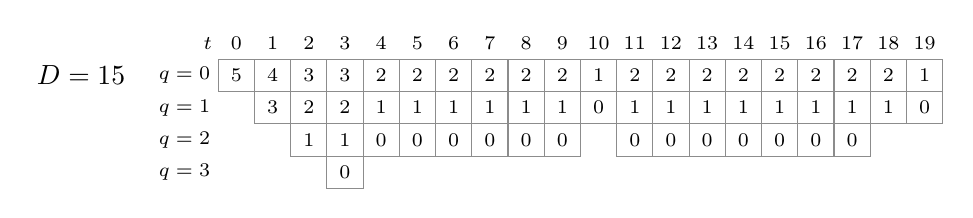
\begin{tikzpicture}[x=.46cm,y=.41cm,baseline=(current bounding box.center)]
\node[anchor=east] at (-2.8,-1) {$D=15$};
\node[anchor=east,font=\scriptsize] at (-.4,0) {$t$};
\node[font=\scriptsize] at (0,0) {$0$};
\node[font=\scriptsize] at (1,0) {$1$};
\node[font=\scriptsize] at (2,0) {$2$};
\node[font=\scriptsize] at (3,0) {$3$};
\node[font=\scriptsize] at (4,0) {$4$};
\node[font=\scriptsize] at (5,0) {$5$};
\node[font=\scriptsize] at (6,0) {$6$};
\node[font=\scriptsize] at (7,0) {$7$};
\node[font=\scriptsize] at (8,0) {$8$};
\node[font=\scriptsize] at (9,0) {$9$};
\node[font=\scriptsize] at (10,0) {$10$};
\node[font=\scriptsize] at (11,0) {$11$};
\node[font=\scriptsize] at (12,0) {$12$};
\node[font=\scriptsize] at (13,0) {$13$};
\node[font=\scriptsize] at (14,0) {$14$};
\node[font=\scriptsize] at (15,0) {$15$};
\node[font=\scriptsize] at (16,0) {$16$};
\node[font=\scriptsize] at (17,0) {$17$};
\node[font=\scriptsize] at (18,0) {$18$};
\node[font=\scriptsize] at (19,0) {$19$};
\node[anchor=east,font=\scriptsize] at (-.45,-1) {$q=0$};
\node[font=\scriptsize,draw=black!45,minimum width=.46cm,minimum height=.41cm,inner sep=0pt] at (0,-1) {$5$};
\node[font=\scriptsize,draw=black!45,minimum width=.46cm,minimum height=.41cm,inner sep=0pt] at (1,-1) {$4$};
\node[font=\scriptsize,draw=black!45,minimum width=.46cm,minimum height=.41cm,inner sep=0pt] at (2,-1) {$3$};
\node[font=\scriptsize,draw=black!45,minimum width=.46cm,minimum height=.41cm,inner sep=0pt] at (3,-1) {$3$};
\node[font=\scriptsize,draw=black!45,minimum width=.46cm,minimum height=.41cm,inner sep=0pt] at (4,-1) {$2$};
\node[font=\scriptsize,draw=black!45,minimum width=.46cm,minimum height=.41cm,inner sep=0pt] at (5,-1) {$2$};
\node[font=\scriptsize,draw=black!45,minimum width=.46cm,minimum height=.41cm,inner sep=0pt] at (6,-1) {$2$};
\node[font=\scriptsize,draw=black!45,minimum width=.46cm,minimum height=.41cm,inner sep=0pt] at (7,-1) {$2$};
\node[font=\scriptsize,draw=black!45,minimum width=.46cm,minimum height=.41cm,inner sep=0pt] at (8,-1) {$2$};
\node[font=\scriptsize,draw=black!45,minimum width=.46cm,minimum height=.41cm,inner sep=0pt] at (9,-1) {$2$};
\node[font=\scriptsize,draw=black!45,minimum width=.46cm,minimum height=.41cm,inner sep=0pt] at (10,-1) {$1$};
\node[font=\scriptsize,draw=black!45,minimum width=.46cm,minimum height=.41cm,inner sep=0pt] at (11,-1) {$2$};
\node[font=\scriptsize,draw=black!45,minimum width=.46cm,minimum height=.41cm,inner sep=0pt] at (12,-1) {$2$};
\node[font=\scriptsize,draw=black!45,minimum width=.46cm,minimum height=.41cm,inner sep=0pt] at (13,-1) {$2$};
\node[font=\scriptsize,draw=black!45,minimum width=.46cm,minimum height=.41cm,inner sep=0pt] at (14,-1) {$2$};
\node[font=\scriptsize,draw=black!45,minimum width=.46cm,minimum height=.41cm,inner sep=0pt] at (15,-1) {$2$};
\node[font=\scriptsize,draw=black!45,minimum width=.46cm,minimum height=.41cm,inner sep=0pt] at (16,-1) {$2$};
\node[font=\scriptsize,draw=black!45,minimum width=.46cm,minimum height=.41cm,inner sep=0pt] at (17,-1) {$2$};
\node[font=\scriptsize,draw=black!45,minimum width=.46cm,minimum height=.41cm,inner sep=0pt] at (18,-1) {$2$};
\node[font=\scriptsize,draw=black!45,minimum width=.46cm,minimum height=.41cm,inner sep=0pt] at (19,-1) {$1$};
\node[anchor=east,font=\scriptsize] at (-.45,-2) {$q=1$};
\node[font=\scriptsize,draw=black!45,minimum width=.46cm,minimum height=.41cm,inner sep=0pt] at (1,-2) {$3$};
\node[font=\scriptsize,draw=black!45,minimum width=.46cm,minimum height=.41cm,inner sep=0pt] at (2,-2) {$2$};
\node[font=\scriptsize,draw=black!45,minimum width=.46cm,minimum height=.41cm,inner sep=0pt] at (3,-2) {$2$};
\node[font=\scriptsize,draw=black!45,minimum width=.46cm,minimum height=.41cm,inner sep=0pt] at (4,-2) {$1$};
\node[font=\scriptsize,draw=black!45,minimum width=.46cm,minimum height=.41cm,inner sep=0pt] at (5,-2) {$1$};
\node[font=\scriptsize,draw=black!45,minimum width=.46cm,minimum height=.41cm,inner sep=0pt] at (6,-2) {$1$};
\node[font=\scriptsize,draw=black!45,minimum width=.46cm,minimum height=.41cm,inner sep=0pt] at (7,-2) {$1$};
\node[font=\scriptsize,draw=black!45,minimum width=.46cm,minimum height=.41cm,inner sep=0pt] at (8,-2) {$1$};
\node[font=\scriptsize,draw=black!45,minimum width=.46cm,minimum height=.41cm,inner sep=0pt] at (9,-2) {$1$};
\node[font=\scriptsize,draw=black!45,minimum width=.46cm,minimum height=.41cm,inner sep=0pt] at (10,-2) {$0$};
\node[font=\scriptsize,draw=black!45,minimum width=.46cm,minimum height=.41cm,inner sep=0pt] at (11,-2) {$1$};
\node[font=\scriptsize,draw=black!45,minimum width=.46cm,minimum height=.41cm,inner sep=0pt] at (12,-2) {$1$};
\node[font=\scriptsize,draw=black!45,minimum width=.46cm,minimum height=.41cm,inner sep=0pt] at (13,-2) {$1$};
\node[font=\scriptsize,draw=black!45,minimum width=.46cm,minimum height=.41cm,inner sep=0pt] at (14,-2) {$1$};
\node[font=\scriptsize,draw=black!45,minimum width=.46cm,minimum height=.41cm,inner sep=0pt] at (15,-2) {$1$};
\node[font=\scriptsize,draw=black!45,minimum width=.46cm,minimum height=.41cm,inner sep=0pt] at (16,-2) {$1$};
\node[font=\scriptsize,draw=black!45,minimum width=.46cm,minimum height=.41cm,inner sep=0pt] at (17,-2) {$1$};
\node[font=\scriptsize,draw=black!45,minimum width=.46cm,minimum height=.41cm,inner sep=0pt] at (18,-2) {$1$};
\node[font=\scriptsize,draw=black!45,minimum width=.46cm,minimum height=.41cm,inner sep=0pt] at (19,-2) {$0$};
\node[anchor=east,font=\scriptsize] at (-.45,-3) {$q=2$};
\node[font=\scriptsize,draw=black!45,minimum width=.46cm,minimum height=.41cm,inner sep=0pt] at (2,-3) {$1$};
\node[font=\scriptsize,draw=black!45,minimum width=.46cm,minimum height=.41cm,inner sep=0pt] at (3,-3) {$1$};
\node[font=\scriptsize,draw=black!45,minimum width=.46cm,minimum height=.41cm,inner sep=0pt] at (4,-3) {$0$};
\node[font=\scriptsize,draw=black!45,minimum width=.46cm,minimum height=.41cm,inner sep=0pt] at (5,-3) {$0$};
\node[font=\scriptsize,draw=black!45,minimum width=.46cm,minimum height=.41cm,inner sep=0pt] at (6,-3) {$0$};
\node[font=\scriptsize,draw=black!45,minimum width=.46cm,minimum height=.41cm,inner sep=0pt] at (7,-3) {$0$};
\node[font=\scriptsize,draw=black!45,minimum width=.46cm,minimum height=.41cm,inner sep=0pt] at (8,-3) {$0$};
\node[font=\scriptsize,draw=black!45,minimum width=.46cm,minimum height=.41cm,inner sep=0pt] at (9,-3) {$0$};
\node[font=\scriptsize,draw=black!45,minimum width=.46cm,minimum height=.41cm,inner sep=0pt] at (11,-3) {$0$};
\node[font=\scriptsize,draw=black!45,minimum width=.46cm,minimum height=.41cm,inner sep=0pt] at (12,-3) {$0$};
\node[font=\scriptsize,draw=black!45,minimum width=.46cm,minimum height=.41cm,inner sep=0pt] at (13,-3) {$0$};
\node[font=\scriptsize,draw=black!45,minimum width=.46cm,minimum height=.41cm,inner sep=0pt] at (14,-3) {$0$};
\node[font=\scriptsize,draw=black!45,minimum width=.46cm,minimum height=.41cm,inner sep=0pt] at (15,-3) {$0$};
\node[font=\scriptsize,draw=black!45,minimum width=.46cm,minimum height=.41cm,inner sep=0pt] at (16,-3) {$0$};
\node[font=\scriptsize,draw=black!45,minimum width=.46cm,minimum height=.41cm,inner sep=0pt] at (17,-3) {$0$};
\node[anchor=east,font=\scriptsize] at (-.45,-4) {$q=3$};
\node[font=\scriptsize,draw=black!45,minimum width=.46cm,minimum height=.41cm,inner sep=0pt] at (3,-4) {$0$};
\end{tikzpicture}
\par\smallskip

\endgroup
\caption{Neighborhoods of an outside vertex at a marked triangle.
For each listed pair $(t,q)$, the entry is the largest retained value of $E$.
A blank cell has no retained triple.}
\label{fig:finite-triangle-profiles}
\end{figure}

A linear inequality holding on this finite
set of triples holds on its convex hull. Multiplying by the
nonnegative weight of the rooted triangle and summing over all its
images gives a linear inequality on the weighted pattern counts.
The integer enumeration and its supporting planes are specified in
Appendix~\ref{app:profile-verification}. When summing extensions for
$t$, the three maps of the fourth position to a root are subtracted.
